\section{Die Navier-Stokes-Gleichungen}

\subsection{Fluide}

Die Gleichungen, die im folgenden beschrieben werden, gelten nicht nur für Gase
wie Luft, sondern auch für Flüssigkeiten wie Wasser. Deshalb wird im Folgenden
der Begriff \PimiddyBegriff{Fluid} verwendet, der beide Zustände zusammenfasst.
Physikalisch gesehen sind Fluide Substanzen, die einer beliebig langsamen
Scherung keinen Widerstand entgegensetzen. Dieses Konzept ist allerdings in
dieser Arbeit nicht von Bedeutung.

Fluide können unter unterschiedlichen Gesichtspunkten modelliert werden, je
nachdem, an welcher Art Fluid man interessiert ist. Auch die äußeren
Gegebenheiten haben Einfluss auf die gewählte Modellierung. Daher soll zunächst
das Modell erläutert werden, bevor die zugehörigen Gleichungen vorgestellt
werden.

Das \emph{Volumen} von Fluiden ist im Allgemeinen nicht konstant, es wird durch
Veränderung von Druck und Dichte beeinflusst. Dies geschieht z.B. beim
Übertreten der Schallmauer (im Medium Luft, beispielsweise bei einer Explosion)
oder bei der Ausbreitung von Tönen unter Wasser. Bei der Modellierung
unterscheidet man zwischen \PimiddyBegriff{komprimierbaren} und
\PimiddyBegriff{unkomprimierbaren} Fluiden, je nachdem, ob die Veränderung des
Volumens eine Rolle für die Simulation spielt.

Es werden hier nur \emph{inkompressible} Fluide betrachtet. Dies stellt kein
Problem dar, da nur vergleichsweise kleine Geschwindigkeiten modelliert werden.
Das Modell wird dadurch allerdings wesentlich vereinfacht.

Zudem haben Fluide im allgemeinen an jedem Punkt eine unterschiedliche
\emph{Dichte} $\rho$. Zur weiteren Vereinfachung wird hier allerdings von einer
konstanten Dichte ausgegangen.

\subsection{Einführung}

Das Modell eines Fluids besteht mathematisch gesehen aus mehreren Feldern
(Skalar- und Vektorfeldern), die den \emph{Zustand} des Fluids zu einem
\emph{Zeitpunkt} $t$ an einer \emph{Position} $\vec{x}$ angeben.

Für die \PimiddyBegriff{Navier-Stokes-Gleichungen}, benannt nach den
Mathematikern \PimiddyName{Claude-Louis Navier} und \PimiddyName{George Gabriel
Stokes}, werden zwei Felder betrachtet, die \emph{Bewegungsgeschwindigkeit}
$\vec{u}(\vec{x},t)$ des Fluids und der \emph{Druck} $p(\vec{x},t)$. Die
Gleichungen lauten wie folgt:

\begin{align}
\label{eq:navier_stokes_momentum_equation}
\frac{
	\partial
	\vec{u}
}
{
	\partial t
} +
\vec{u} \PimiddyDiv \vec{u}
& =
\vec{g} +
\nu \PimiddyLaplace \vec{u} -
\frac{
	1
}
{
	\rho
}
\PimiddyGrad p
\\
\label{eq:navier_stokes_incompressibility_condition}
\PimiddyDiv \vec{u} & = 0
\end{align}

\autoref{eq:navier_stokes_momentum_equation} ist eine Differentialgleichung, die
wegen des Terms $\vec{u} \PimiddyDiv \vec{u}$ nichtlinear ist. Das macht sie
besonders schwer mit klassischen Verfahren lösbar.

Die Dimension des Raums taucht in den Gleichungen nicht auf, man kann sie also
in zwei oder drei Dimensionen betrachten. Zur Veranschaulichung wird im
Folgenden oft von zwei Dimensionen ausgegangen.

Die einzelnen Bestandteile werden in den folgenden Kapiteln genauer beleuchtet,
hier soll allerdings schon ein kurzer Überblick gegeben werden:

\begin{itemize}
\item
	Die Konstante $\rho$ gibt die \emph{Dichte} des Fluids an. Für Wasser beträgt
	sie etwa $1000 \frac{kg}{m^3}$, für Luft etwa $1.3 \frac{kg}{m^3}$
	(\cite{Bridson2007}).
\item
	Der \emph{Druck} spielt bei den späteren Berechnungen eine große Rolle.
	Er ist dort besonders hoch, wo das Fluid auf Hindernisse trifft.
\item
	Kräfte, die von außen auf das Fluid wirken, wie z.B. die Schwerkraft
	oder auch der eingeführte Wind, werden im Vektorfeld $\vec{g} \colon
	\PimiddyReell^3 \to \PimiddyReell^3$ zusammengefasst.
\item
	Schließlich unterscheiden sich Fluide in ihrer \PimiddyBegriff{Viskosität} oder
	\PimiddyQuotes{Zähflüssigkeit}, die in der Gleichung mit $\nu$ bezeichnet ist.
	Dickflüssige Fluide wie Honig haben ein hohes $\nu$, dünnflüssige wie Luft ein
	niedriges $\nu$.
\end{itemize}

\autoref{eq:navier_stokes_momentum_equation} wird
\PimiddyBegriff{Impulsgleichung} genannt,
\autoref{eq:navier_stokes_incompressibility_condition} nennt man
\PimiddyBegriff{Unkomprimierbarkeitsbedingung}. Der Name und die Bedeutung der
Gleichungen werden im Folgenden näher beleuchtet.

Die Navier-Stokes-Gleichungen komplett zu erläutern geht über den Rahmen dieser
Arbeit weit hinaus, daher soll vor allem ein intuitives Verständnis der
einzelnen Bestandteile gegeben werden. Außerdem soll eine Beziehung zur
klassischen Mechanik hergestellt werden, da die Gleichungen starke Parallelen
hierzu aufweisen.

\subsection{Die Impulsgleichung}

\subsubsection{Lagrange und Euler}

Um Fluide zu modellieren, gibt es zwei Betrachtungsweisen. Die
\PimiddyBegriff{Euler'sche-Betrachtungsweise} und die
\PimiddyBegriff{Lagrange'sche-Betrachtungsweise}.

Bei der \emph{Lagrange'schen-Betrachtungsweise} modelliert man das Fluid als System
von mikroskopisch kleinen \emph{Partikeln} (man modelliert sozusagen die
Moleküle des Fluids einzeln). Jedes Partikel hat ein Volumen $V$, eine
Masse $m$, eine Position $\vec{x}$ und eine Geschwindigkeit $\vec{u}$. In jedem
Simulationsschritt berechnet man die Kräfte, die auf die Partikel wirken, und
berechnet die resultierende Beschelunigung mit der Newton'schen Formel:

\begin{align*}
m \cdot \vec{a} &= \vec{F} \\
m \cdot \frac{\partial \vec{u}}{\partial t} &= \vec{F}
\end{align*}

Diese Vorgehensweise ist intuitiv und einfach umzusetzen, aber mathematisch
schwer zu analysieren. Beispielsweise kann man die Frage \PimiddyQuotes{Welche
Geschwindigkeit hat das Fluid an Position $\vec{x}$?} nicht sofort
beantworten.

Bei der \emph{Euler'schen-Betrachtungsweise} hingegen hält man jeweils einen Punkt im
Raum fest und analysiert das Strömungsverhalten (Geschwindigkeit, Temperatur)
durch diesen Punkt. Diese Art der Modellierung ist weniger intuitiv, lässt sich
mit Hilfe von Vektorfeldern und Skalarfeldern aber sehr gut mathematisch erfassen.

\subsubsection{Die substantielle Ableitung}

\begin{figure}[ht]
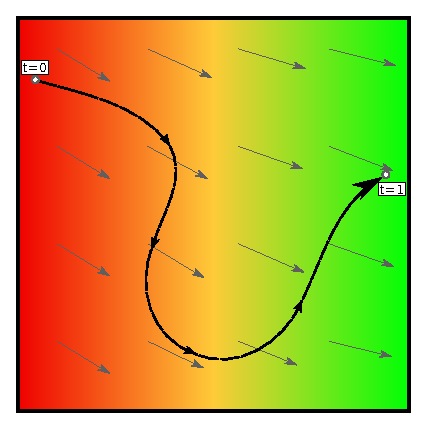
\includegraphics[width=6cm]{images/swimmer_in_water}
\caption{Die Bahn eines Fischs im Wasser. Die Temperatur des Fluids ist hier durch Farben kodiert. Rot bedeutet warmes Wasser, blau bedeutet kaltes Wasser. Nicht dargestellt ist die Veränderung der Wassertemperatur über die Zeit und die Fließrichtung des Wassers. Die Geschwindigkeit des Gewässers wird fürs erste außer Acht gelassen.}
\end{figure}

Sowohl die Euler'sche- als auch die Lagrang'sche Betrachtungsweise spiegeln sich
in den Navier-Stokes-Gleichungen wider. Sie bilden eine Entsprechung der
Gleichung $\vec{F} = m \cdot \vec{a}$ mit dem Unterschied, dass keine Kraft auf
einen einzelnen Körper berechnet wird, sondern auf einen Raumabschnitt (
ein \PimiddyQuotes{Kontinuum}).

Was die beiden Betrachtungsweisen verbindet, ist die
\PimiddyBegriff{substantielle Ableitung}. Zur Herleitung dieser Ableitungsform
betrachten wir zunächst eine beliebige Größe $q(\vec{x},t)$. Dies kann eine
skalare Größe wie z.B. die Temperatur eines Gewässers sein oder eine Vektorgröße
wie die Farbe des Wassers an einem Punkt. Sie ist eine Lagrange'sche Größe, ist
also in jedem Punkt $\vec{x}$ und in jedem Zeitpunkt $t$ gegeben.

Zudem betrachten wir ein Partikel mit einer Bewegungsbahn durch das Fluid (z.B.
einen Fisch im Wasser). Seine Position zum Zeitpunkt $t$ sei gegeben durch
$\vec{p}(t)$. Dies entspricht einer Euler'schen Größe.

Setzen wir beide Größen zusammen, erhalten wir beispielsweise die Temperatur des
Wassers auf der Bahn, die der Fisch im Wasser verfolgt:

\begin{equation}
\PimiddyFormelText{Temperatur}(t) = q(\vec{p}(t),t)
\end{equation}

Wollen wir wissen, wie sich die Umgebungstemperatur des Fischs im Lauf der Zeit
verändert, bilden wir die (totale) Ableitung dieser zusammengesetzten Größe:

\begin{equation}
\frac{
	\partial \PimiddyFormelText{Temperatur}(t)
}
{
	\partial t
}
=
\frac{
	\partial q
}
{
	\partial t
}
+
\PimiddyGrad q \cdot
\frac{
	\partial \vec{p}}
{
	\partial t
}
\end{equation}

Die Summe auf der rechten Seite besteht aus zwei Teilen. Der erste Term,
$\frac{\partial q}{\partial t}$, gibt an, wie sich das Fluid unabhängig von
der Position verändert. Bezogen auf den Fisch gibt dieser Term an, wie
sich die Temperatur des Gewässers über den Tag verteilt verändert. Der
zweite Term ergänzt die Temperaturveränderungen, die durch die Bahn des
Fischs verursacht werden.

Statt eines beliebigen Pfades durch das Fluid nimmt man zur Definition der
substantiellen Ableitung nun das Geschwindigkeitsfeld des Fluids zur Hilfe:

\begin{equation}
\frac{
	Dq}
{
	Dt
} :=
\frac{
	\partial q
}
{
	\partial t
}
+
\PimiddyGrad q \cdot
\vec{u}
\end{equation}

Man geht also von einem Partikel aus, was sich im Fluid \PimiddyQuotes{treiben}
lässt, und misst die Veränderung der Größe $q$ auf seiner Bahn. Analog ist die
substantielle Ableitung für Vektorgrößen definiert:

\begin{equation}
\frac{
	D\vec{q}}
{
	Dt
} :=
\frac{
	\partial q
}
{
	\partial t
}
+
\PimiddyDiv q \cdot
\vec{u}
\end{equation}

Die Impulsgleichung lässt sich mit Hilfe der substantiellen Ableitung so schreiben:

\begin{equation}
\rho \frac{D\vec{u}}{Dt} = - \PimiddyGrad p + \PimiddyLaplace \vec{u} + \vec{f}
\end{equation}

Dies entspricht der klassischen Newton'schen Kraftformel, wobei die Masse $m$
durch die Dichte $\rho$ ersetzt wird\PimiddyFootnote{Die Dichte ist eigentlich
ebenfalls abhängig von Zeit und Position, also $\rho(\vec{x},t)$, wir
beschränken uns allerdings ohne Einschränkungen auf ein einfacheres
Modell.}. Auf der rechten Seite der Gleichung stehen die Kräfte, die das
Fluid beeinflussen. Diese Kräfte sollen im Einzelnen näher beschrieben
werden.

\subsubsection{Die Kräfte in den Navier-Stokes-Gleichungen}

Die Kraft, die überall im Fluid in gleicher Weise wirkt, ist die Schwerkraft:

\begin{equation}
F_g =
\left(
\begin{array}{c}
0 \\
-g \\
0
\end{array}
\right)
\end{equation}

mit $g \cong 9.81 \frac{m}{s^2}$.

Durch den Druck innerhalb des Fluids wird eine weitere Kraft $F_p$ ausgeübt.
Allerdings erzeugt Druck allein keine Veränderung. Ist er über das Fluid
konstant, ist die ausgeübte Kraft gleich 0. Stattdessen wirkt die Kraft $F_p$
\PimiddyQuotes{ausgleichend}. Sie zeigt von Regionen hohen Drucks hin zu
Regionen niedrigeren Drucks. Mathematisch gesehen ist sie also proportional zum
negativen Gradient des Drucks (siehe
\autoref{fig:navier_stokes_particle_system_wall_collision}):

\begin{equation}
\label{eq:navier_stokes_f_p}
F_p = -\PimiddyGrad p
\end{equation}

In den späteren Berechnungen spielt der Druck insbesondere eine Rolle, um das
Fluid in seinem inkompressiblen Zustand zu halten und um das Hineinfließen in
Hindernisse zu verhindern.

\begin{figure}[ht]
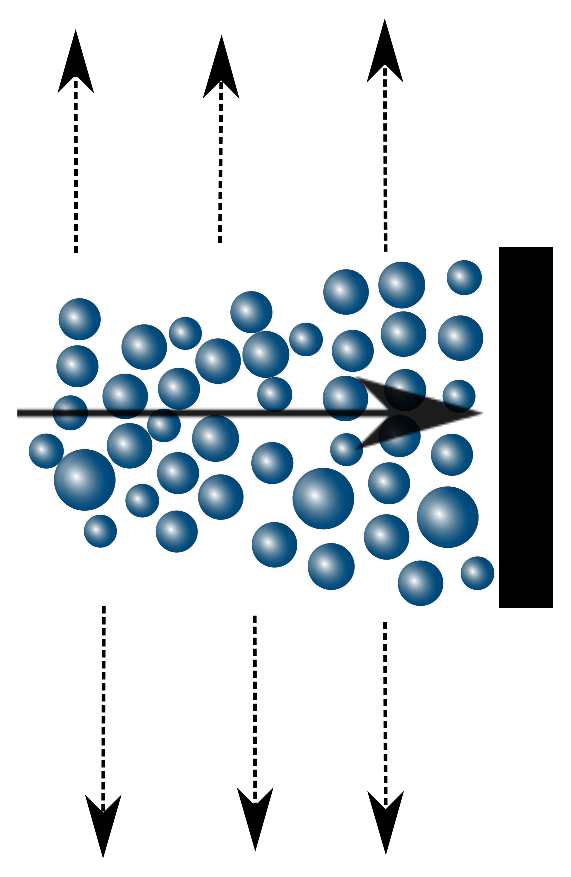
\includegraphics[width=6cm]{images/particle_system_wall_collision}
\caption{Partikelsystem, was auf ein Hindernis prallt. Der durchgezogene Pfeil deutet die Flussrichtung an, die gestrichelten Pfeile den negativen Gradienten des Drucks. Die Partikel erfahren also eine Kraft nach außen.}
\label{fig:navier_stokes_particle_system_wall_collision}
\end{figure}

Die Viskosität des Fluids hat ebenfalls Einfluss auf das Fluid. Bei einem
viskosen Fluid wird jeder Deformation ein Widerstand entgegengesetzt. Eine
Flüssigkeit wie Honig, die um ein Hindernis herumfließt, bildet hinter dem
Hindernis keine Verwirbelungen; die hohe Viskosität wirkt dem entgegen. Luft
hingegen hat eine niedrige Viskosität, bildet also viele Wirbel.

\PimiddyTodo{Hier ein Bild von Honig vs. Luft (oder Wasser)}

Die Kraft, die durch die Viskosität ausgeübt wird, hat den Effekt,
Geschwindigkeitsunterschiede innerhalb des Fluids auszugleichen. Sie ist
daher proportional zum Laplace der Geschwindigkeit:

\begin{equation}
\label{eq:navier_stokes_f_v}
F_v = \mu \cdot \PimiddyLaplace \vec{u}
\end{equation}

Die Konstante $\mu$ stellt die \PimiddyBegriff{dynamische Viskosität} des Fluids
dar.

\subsection{Die Unkomprimierbarkeitsbedingung}
\label{sec:mathematics_incompressibility_condition_section}

\begin{figure}[ht]
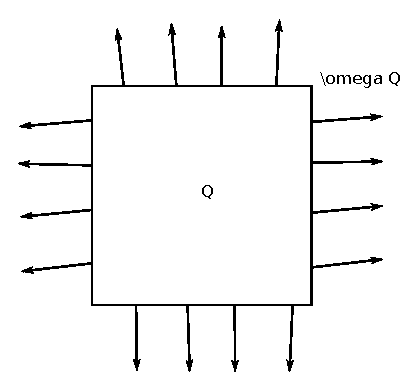
\includegraphics[width=6cm]{images/incompressibility_condition_example}
\caption{Fluss durch einen Würfel (Querschnitt)}
\end{figure}

Um die Unkomprimierbarkeitsbedingung zu motivieren, sei ein beliebiges Volumen
$\Omega \subset \PimiddyReell^3$ gegeben, z.B. ein Würfel im Raum. Seine
Oberfläche sei $\partial \Omega$.

Die Änderung des Würfelvolumens über die Zeit kann berechnet werden, indem man
über die Normalenkomponente entlang seiner Oberfläche integriert \cite{Chorin1980}. Bildlich
gesprochen summiert man auf diese Weise eingehende und ausgehende Strömungen an
den Würfelseitenflächen:

\begin{equation}
\frac{
	\partial \PimiddyFormelText{Volumen}(\Omega)
}
{
	\partial t
}
=
\iint_{\partial \Omega} \vec{u} \cdot n
\end{equation}

Damit die Flüssigkeit unkomprimierbar ist, sollte dieses Integral verschwinden:

\begin{equation}
\iint_{\partial \Omega} \vec{u} \cdot n = 0
\end{equation}

Mit Hilfe des Divergenzsatzes können wir dieses Integral in ein Volumenintegral
umformen:

\begin{equation}
\iiint_\Omega \PimiddyDiv \vec{u} = 0
\end{equation}

Da $\Omega$ beliebig gewählt war, folgt $\PimiddyDiv \vec{u} = 0$.

\PimiddyTodo{Hier noch etwas über Wirbelbildung sagen, vielleicht das Bild bringen, wo Wirbel durch den Projektionsoperator entstehen.}
